\documentclass[11pt, conference, onecolumn]{IEEEtran}
\IEEEoverridecommandlockouts
\usepackage{amsmath,amssymb,amsfonts}
\usepackage{graphicx}
\usepackage{textcomp}
\usepackage{xcolor}
\usepackage{algorithm,algpseudocode}
\algrenewcommand\algorithmicindent{0.9em}%
\usepackage{soul}
\usepackage{xspace}
\usepackage{subfigure}
\pagestyle{plain}
\DeclareMathOperator*{\argminA}{arg\,min} % Jan Hlavacek
\DeclareMathOperator*{\argmaxA}{arg\,max} % Jan Hlavacek

\newcommand{\todo}[1]{\color{red}\textbf{\hl{#1}}\color{black}\xspace}
%\newcommand{\todo}[1]{}
\newcommand{\rom}[1]{\expandafter{\romannumeral #1\relax}}

\def\BibTeX{{\rm B\kern-.05em{\sc i\kern-.025em b}\kern-.08em
    T\kern-.1667em\lower.7ex\hbox{E}\kern-.125emX}}
\begin{document}

\title{Branch and Bound: Minimize Maximum Stretch time during Process Scheduling}

\author{
Md Maruf Hossain \\
Kyle Tibbetts \\
Anirudh Narayana \\
}

\maketitle
\section{PROBLEM}


\textbf{Input}: $n$ tasks of processing time $p_i$ to schedule on one processor and release time $r_i$. 
%\begin{equation*}
%T = (  t_1, t_2 . . . ., , t_n  ) , \text{ where }  t_i = (p_i, r_i) 
%\end{equation*}


\textbf{Output}: For each task, a start time $\sigma_i \geq 0$. Task $i$ can not start before it is released: $\sigma_i \geq r_i$. Task $i$ completes at $C_i = \sigma_i + p_i$. No two tasks can be excuting at the same time: $\forall i,j [\sigma_i;C_i[ \cap [\sigma_j;C_j[ = \emptyset $ \\ 

\textbf{Metric}: The flow time of a task is the time that elapsed between its release and completion: $F_i = C_i - r_i$. The stretch of a task is its Flow time normalized by its processing time: $S_i = \frac{F_i}{p_i}$. Minimize maximum stretch: $S_{max} = max_i S_i$


\section{Importance of the Problem}

This problem performs the task of taking into consideration flow time, and processing time, which will account for time taken of a process and the resulting schedule designed will be more efficient. The following are applications of this problem:
\begin{itemize}
    \item Scheduling transport of goods in large industries.
    \item Minimizing total cost of a telecommunication networks by optimizing topology.
    
    (An expanded case of this problem).
    \item Production Planning.
\end{itemize}

\section{Subsets and Partitioning}
The subsets of the problem is the permutation of the tasks. 
\begin{equation*}
\begin{array}{l}
S\ = T! \qquad\qquad\text{Where } T =\{t_1,\dots,t_n\}
\end{array}
\end{equation*}
We can partition the set $S$ into $n$ subsets where,
\begin{equation*}
\begin{array}{l}
S\ = S_1\cup S_2\cup \dots\cup S_n \qquad\qquad \text{Where }S_i = \{ (t_i,) + T'\ |\  \forall \ T' \in (T \setminus t_i)! \}
\end{array}
\end{equation*}
Each subsets represents all the sequence where a specific task is scheduled first.
Let's say, we have 3 tasks($p_1,p_2,p_3$) then we can get possible 6 different schedule,
\begin{enumerate}
\item $\{p_1\rightarrow p_2\rightarrow  p_3\}$
\item $\{p_1\rightarrow  p_3\rightarrow  p_2\}$
\item $\{p_2\rightarrow  p_1\rightarrow  p_3\}$
\item $\{p_2\rightarrow  p_3\rightarrow  p_1\}$
\item $\{p_3\rightarrow  p_1\rightarrow  p_2\}$
\item $\{p_3\rightarrow  p_2\rightarrow  p_1\}$ 
\end{enumerate}
We are going to divide them into three subsets, $S_1=\{1,2\},\ S_2=\{3,4\} \text{ and } S_3=\{5,6\}$
\section{Approach}
We are after an ordering of the tasks. Given an ordering the start times can be found by $ \sigma_i = max \{ C_{i-1}, r_i \}$ where $C_0 = 0 $

\section{Partition Order}
In this problem, release time and length of the process is the key point to minimize the max stretch of the scheduling. 
If we choose a partition where the release time of the first process is smaller compare to others then it can converge to 
the optimal solution faster.

\begin{equation*}
\begin{array}{l}
\text{explore }S_i \ \text{branch before } S_j\ \text{if }  r_{i}\leq r_{j} 
\end{array}
\end{equation*}

\section{Bound and Relaxations}
In this problem, we have $n$ different sets that can generate $n!$ different max stretch for the scheduling. We are going to maintain 
one global variable $S_{gmin}$ for all and one local variable $S_{lmax}$ for each branch to maintain the bound. 
Here $S_{gmin}$  always holds the global minimum max-stretch and local $S_{lmax}$ only holds the maximum stretch 
of a particular branch.
We are going to once initialize the $S_{gmin}$
\begin{equation*}
\begin{array}{l}
S_{gmin} = \frac{\sum_{i=0}^{n}p_i - min_{i\in\{1,\dots,n\}}r_i}{min_{i\in\{1,\dots,n\}}p_i}
\end{array}
\end{equation*}
On the other hand $S_{lmax}$ will be initialized with $0$ for every branch and in every depth of the tree it will update to maintain the 
max stretch of that branch. A branch will be pruned if $S_{lmax}\geq S_{gmin}$.  If a branch reach at the leaf then it will update 
$S_{gmin} = min\{S_{gmin}, S_{lmax}\}$. 

\section{Traversal Order and Optimal Solution}
Solution always follow the depth first search(DFS) traversal mechanism. But in every depth, if the immediate next branches has the processes 
with the same release time then it always traverse the branch first that contain smaller process time. 
\begin{figure}
\centering
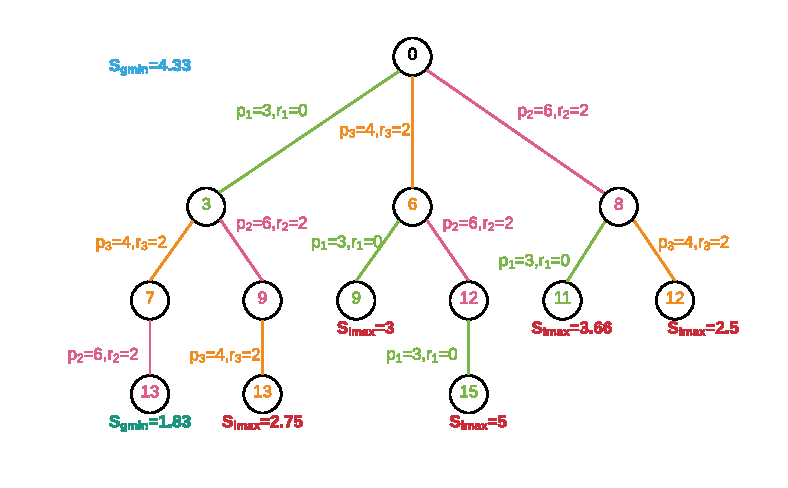
\includegraphics[width=0.96\linewidth]{schedule.pdf}
\caption{Consider 3 process $p_1=3,p_2=6,p_3=4$ with release time $r_1=0,r_2=2,r_3=2$ need to schedule in a system where no two job can schedule at  a time.}
\end{figure}
\section{Weak Dominance Properties}

There exists an optimal solution such that if two tasks have the same release time then always schedule the job with the smaller process time first. If $r_i=r_j=t_r$ and $p_i<p_j$ then if we schedule
$p_i$ first at start time $t_{\sigma}$, 
\begin{equation}
\begin{array}{l}
S_{i} = \frac{t_{\sigma} + p_i - t_r}{p_i} \\
S_{j} = \frac{t_{\sigma} + p_i + p_j- t_r}{p_j} 
\end{array}
\end{equation}
Now if schedule $p_j$ before $p_i$
\begin{equation}
\begin{array}{l}
S'_{j} = \frac{t_{\sigma} + p_j - t_r}{p_j} \\
S'_{i} = \frac{t_{\sigma} + p_i + p_j- t_r}{p_i} 
\end{array}
\end{equation}
Here, $S'_{j} < S_{j}$ but $S'_{i}$ is greater than both $S_{i}$ and $S_{j}$. So, Schedule the smaller job with 
same release time can give better result.

There exists an optimal solution such that tasks are scheduled with no idle time.




\end{document}

